\section{Introduction}\label{s:intro}

% Abstract
This chapter considers the problem of obtaining dense 3D reconstructions of articulated subjects from single and partially occluded views. Humans generally have no problem in predicting, at least approximately, the 3D structure of most scenes including the pose and shape of animals or other people, even from a single view.
However, the visual evidence available in a single 2D image notoriously~\citep{Faugeras01geometry} contains insufficient information for the third dimension to be recovered uniquely. 
This chapter follows a growing body of work that views 3D reconstruction of articulated subjects in a probabilistic setting, and proposes that the goal of reconstructio methods should be to make the posterior distribution as sharp as possible by learning an strong prior on the space of possible solutions. 
In particular, the method described in this chapter recovers \emph{several} plausible and diverse 3D reconstructions which are compatible with the input data. This is implemented using a novel multi-hypothesis neural network architecture, trained using a best-of-M loss where each of the $M$ hypotheses is constrained to lie on a manifold of plausible poses by means of a generative model. Various improvements are suggested to the standard best-of-$M$ setup, to produce reconstruction sets of an arbitrary size, ensuring these are plausible and diverse with a learnt normalizing flow prior and discouraging mode degeneration with a multi-hypothesis reprojection loss.
A fundamental insight relied upon is that ambiguities in 3D body poses can be effectively modelled using a similar parameterization as in previous chapters, using a suitable 3D morphable model.
As well as being the first system capable of modelling ambiguities in 3D animal reconstruction, the method is shown to outperform alternative approaches in ambiguous pose recovery on standard benchmarks for 3D humans and in heavily occluded versions of these benchmarks. The chapter begins by introducing key concepts relied upon in this chapter, as well as discussing the related literature. 

\begin{figure}
\setlength{\fboxsep}{0pt}%
\setlength{\fboxrule}{0pt}%
\centering{\begin{tabular}{@{}c@{}}
    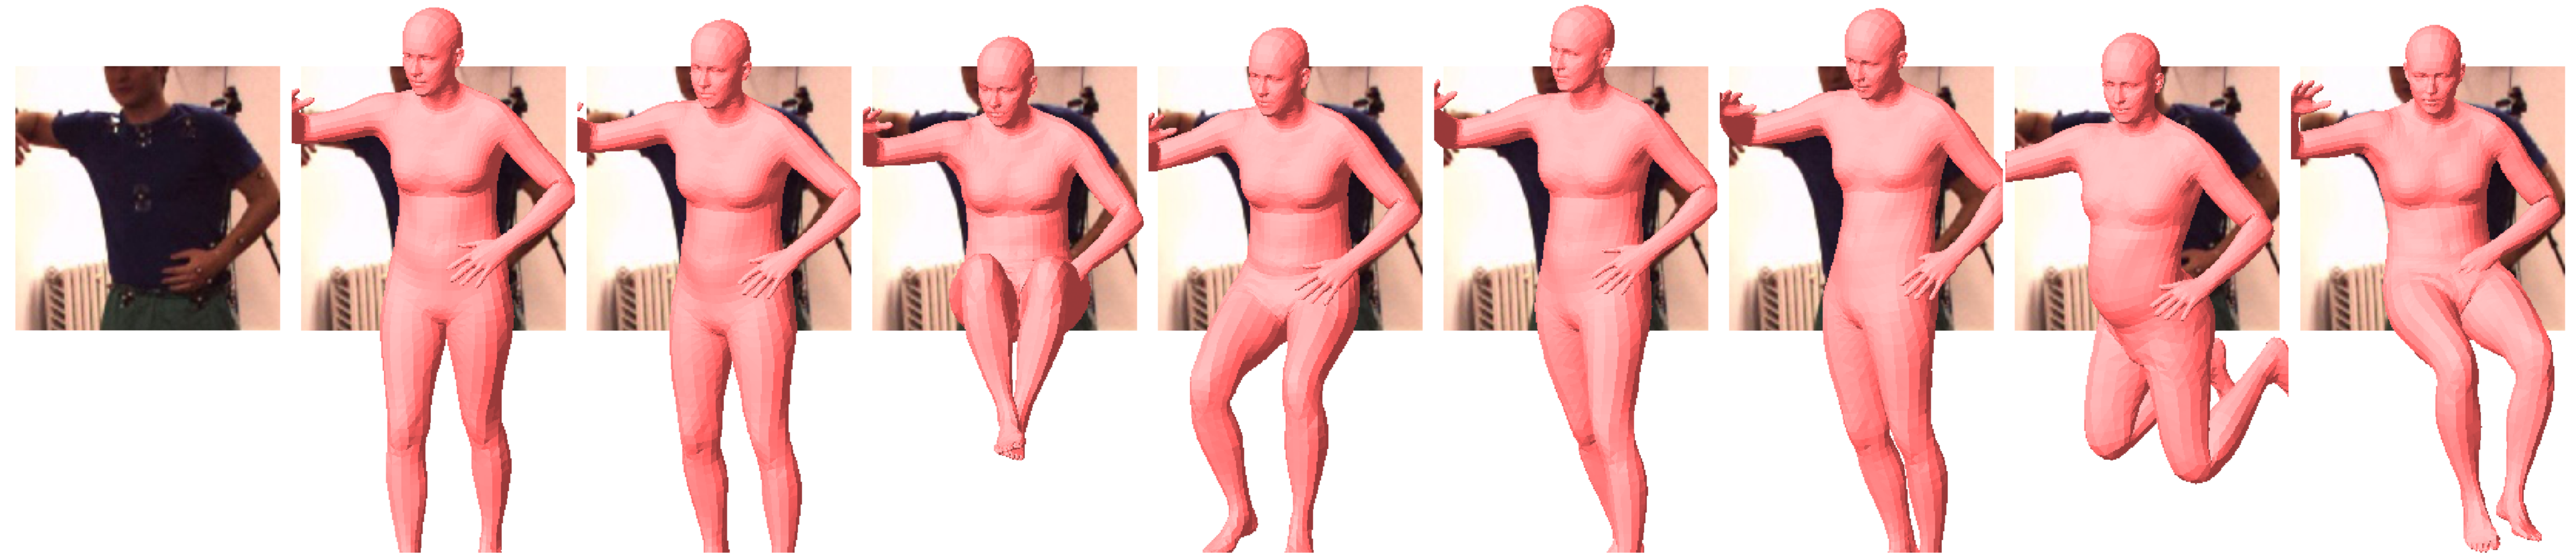
\includegraphics[width=0.49\linewidth,trim=4 8 8 10,clip]{splash/sample_2.pdf} 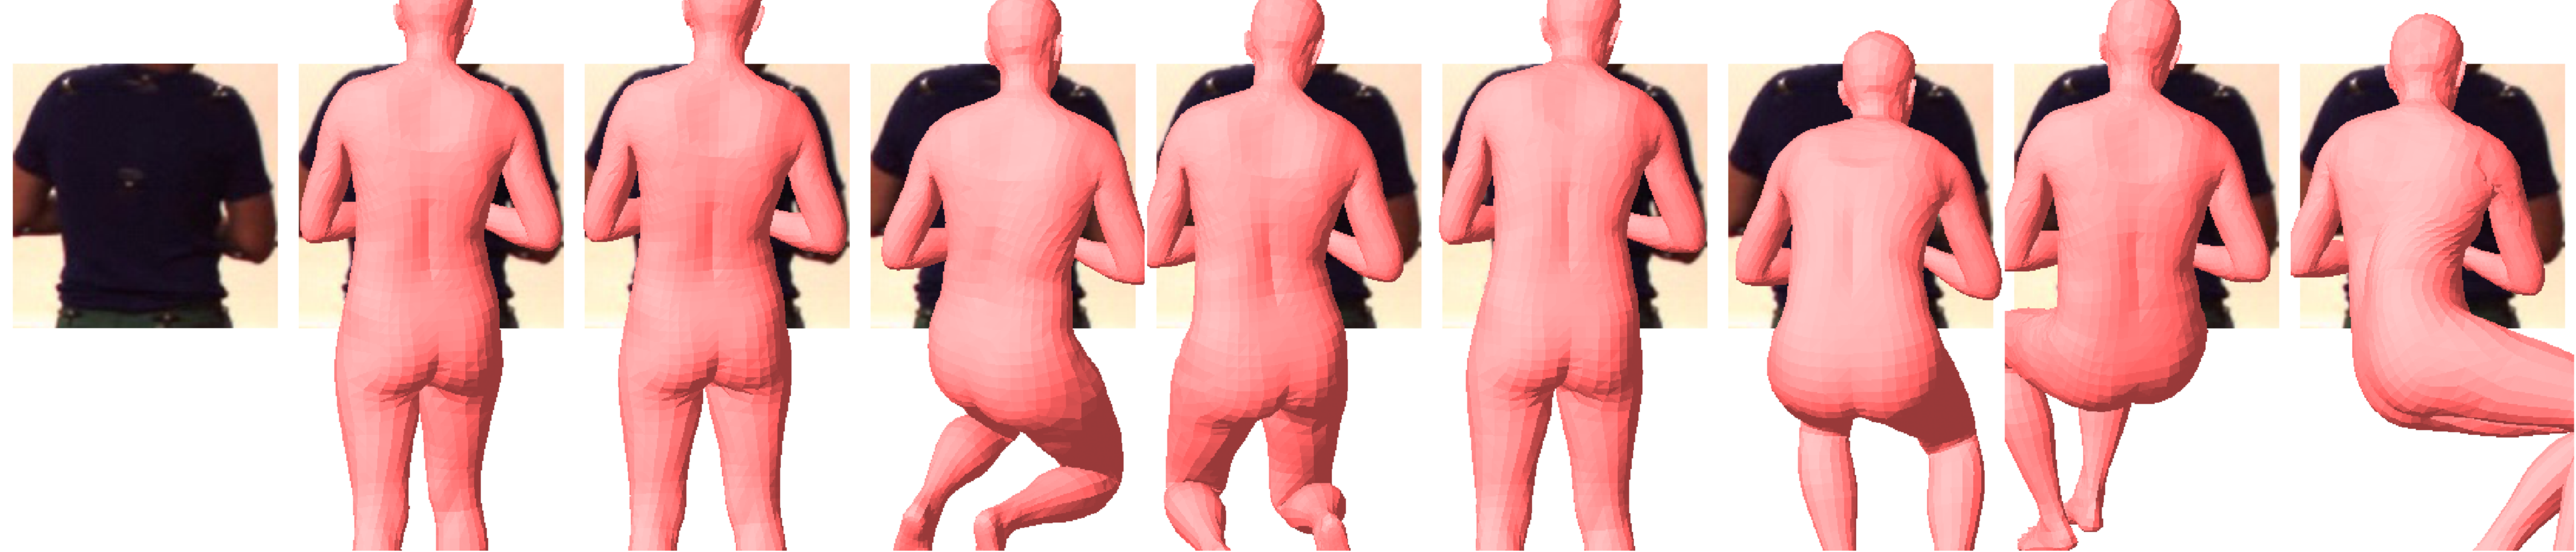
\includegraphics[width=0.49\linewidth,trim=4 8 8 10,clip]{splash/sample_7.pdf}\\
    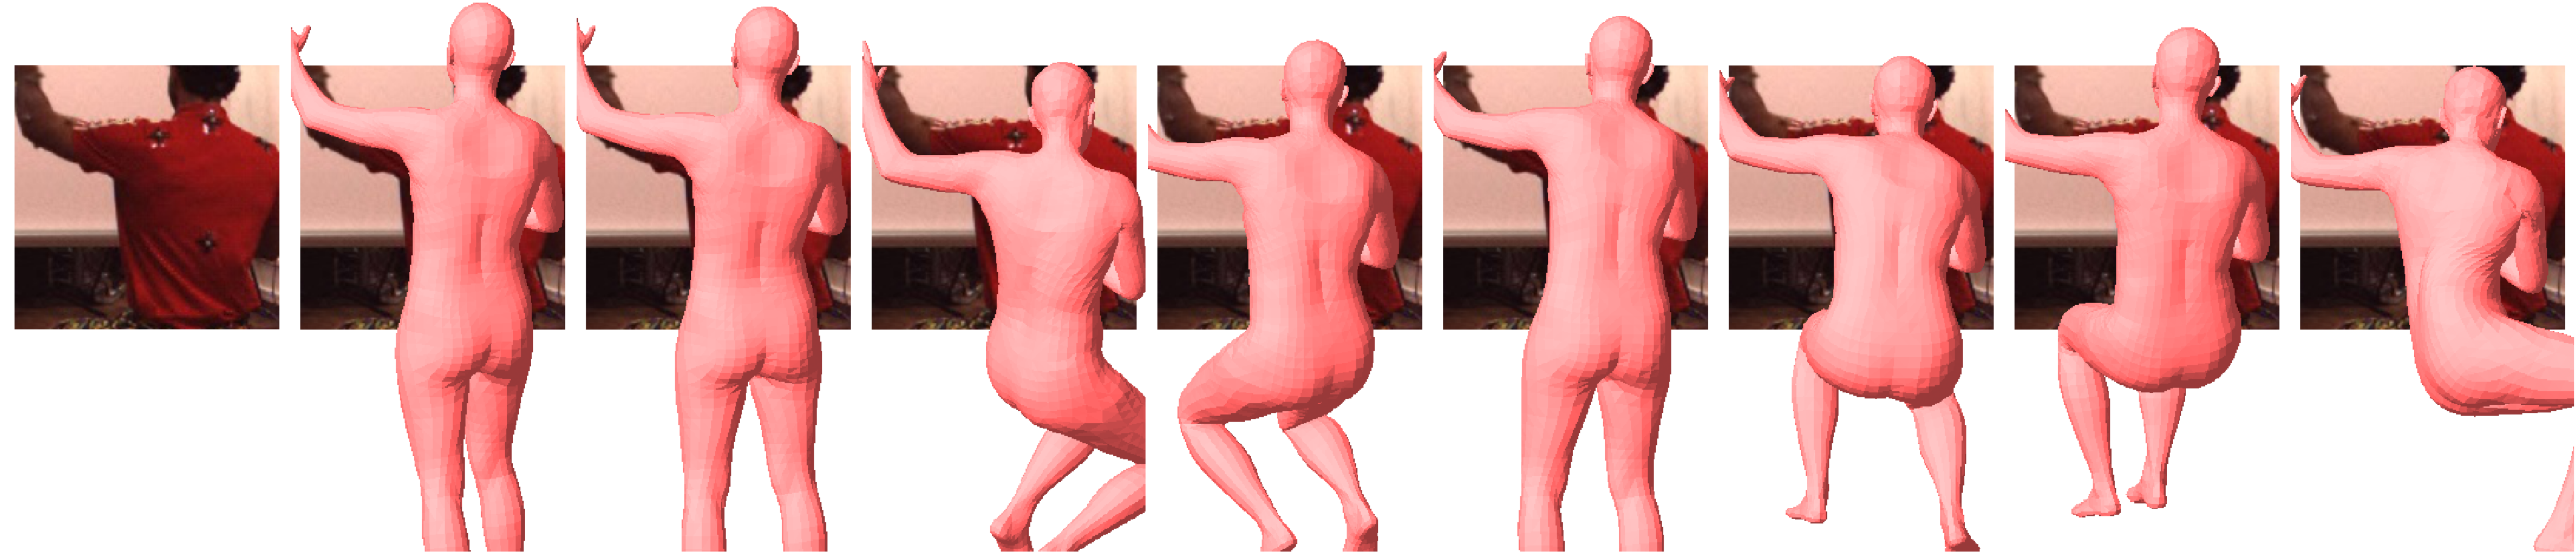
\includegraphics[width=0.49\linewidth,trim=8 10 10 12,clip]{splash/sample_8.pdf} 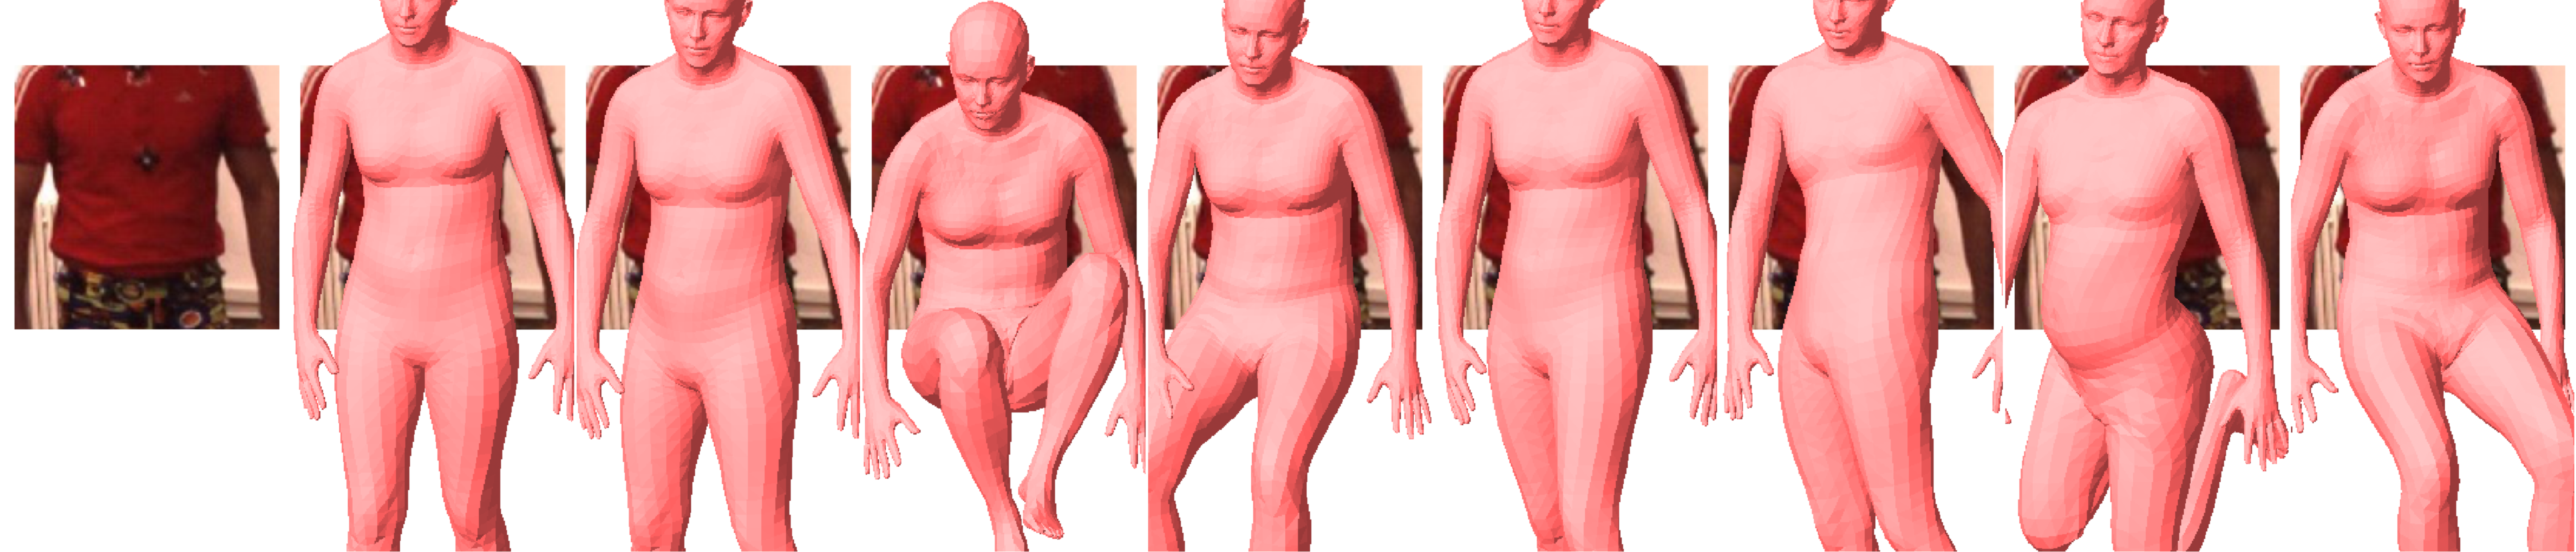
\includegraphics[width=0.49\linewidth,trim=8 10 10  10,clip]{splash/sample_13.pdf}
\end{tabular}}
\captionof{figure}{
\textbf{Human mesh recovery in an ambiguous setting.}
We propose a novel method that, given an occluded input image of a person, outputs the set of meshes which constitute plausible human bodies that are consistent with the partial view.
The ambiguous poses are predicted using a novel $n$-quantized-best-of-$M$ method.\label{fig:splash}}
\end{figure}


\subsection{Limitations of state-of-the-art 3D reconstruction techniques}

Recent progress in single-view 3D model reconstruction for articulated subjects has been impressive.
Methods such as HMR~\citep{kanazawa18end-to-end}, GraphCMR~\citep{kolotouros19convolutional} and SPIN~\citep{kolotouros19learning} for humans and 3D-Safari~\cite{xxx} and the work in \Cref{chap:wldo} for animals, formulate the task as learning a deep neural network that maps 2D images to the parameters of a 3D morphable model (usually SMAL~\cite{zuffi2017menagerie} for animals or SMPL~\cite{loper15smpl} for humans).
Although these method work well in general, they are not immune from failures~(\cref{fig:issues}).
Their main weakness is when processing \emph{heavily occluded images} of the object.
When a large part of the object is missing, say the hind legs of an animal or lower body of a sitting human, they output reconstructions that are often implausible.
Since these approaches produce only one hypothesis as output, they very likely learn to approximate the mean of the posterior distribution, which may not correspond to any plausible pose.
A simple thought experiment helps provide insight behind this suboptimality. Consider an agent which reaches a lake and must randomly decide between travelling left or right around. % TODO: continue this.
Unfortunately, this failure modality is rather common in animal scenes due to environmental and self-occlusion and also for human imagery, for example from scene clutter and crowds.

% Discuss other approaches for dealing with this limitation
This chapter considers the challenge of recovering 3D mesh reconstructions of complex articulated objects such as humans from highly ambiguous image data, often containing significant occlusions of the object.
Clearly, it is generally impossible to reconstruct the object uniquely if too much evidence is missing; however, it is still possible to predict a \emph{set} containing all possible reconstructions (see \cref{fig:splash}).
While ambiguous pose reconstruction has been previously investigated, this work proposes the first deep learning approach for ambiguous reconstructions of the \emph{full animal/human mesh}.

\begin{figure}[t]
    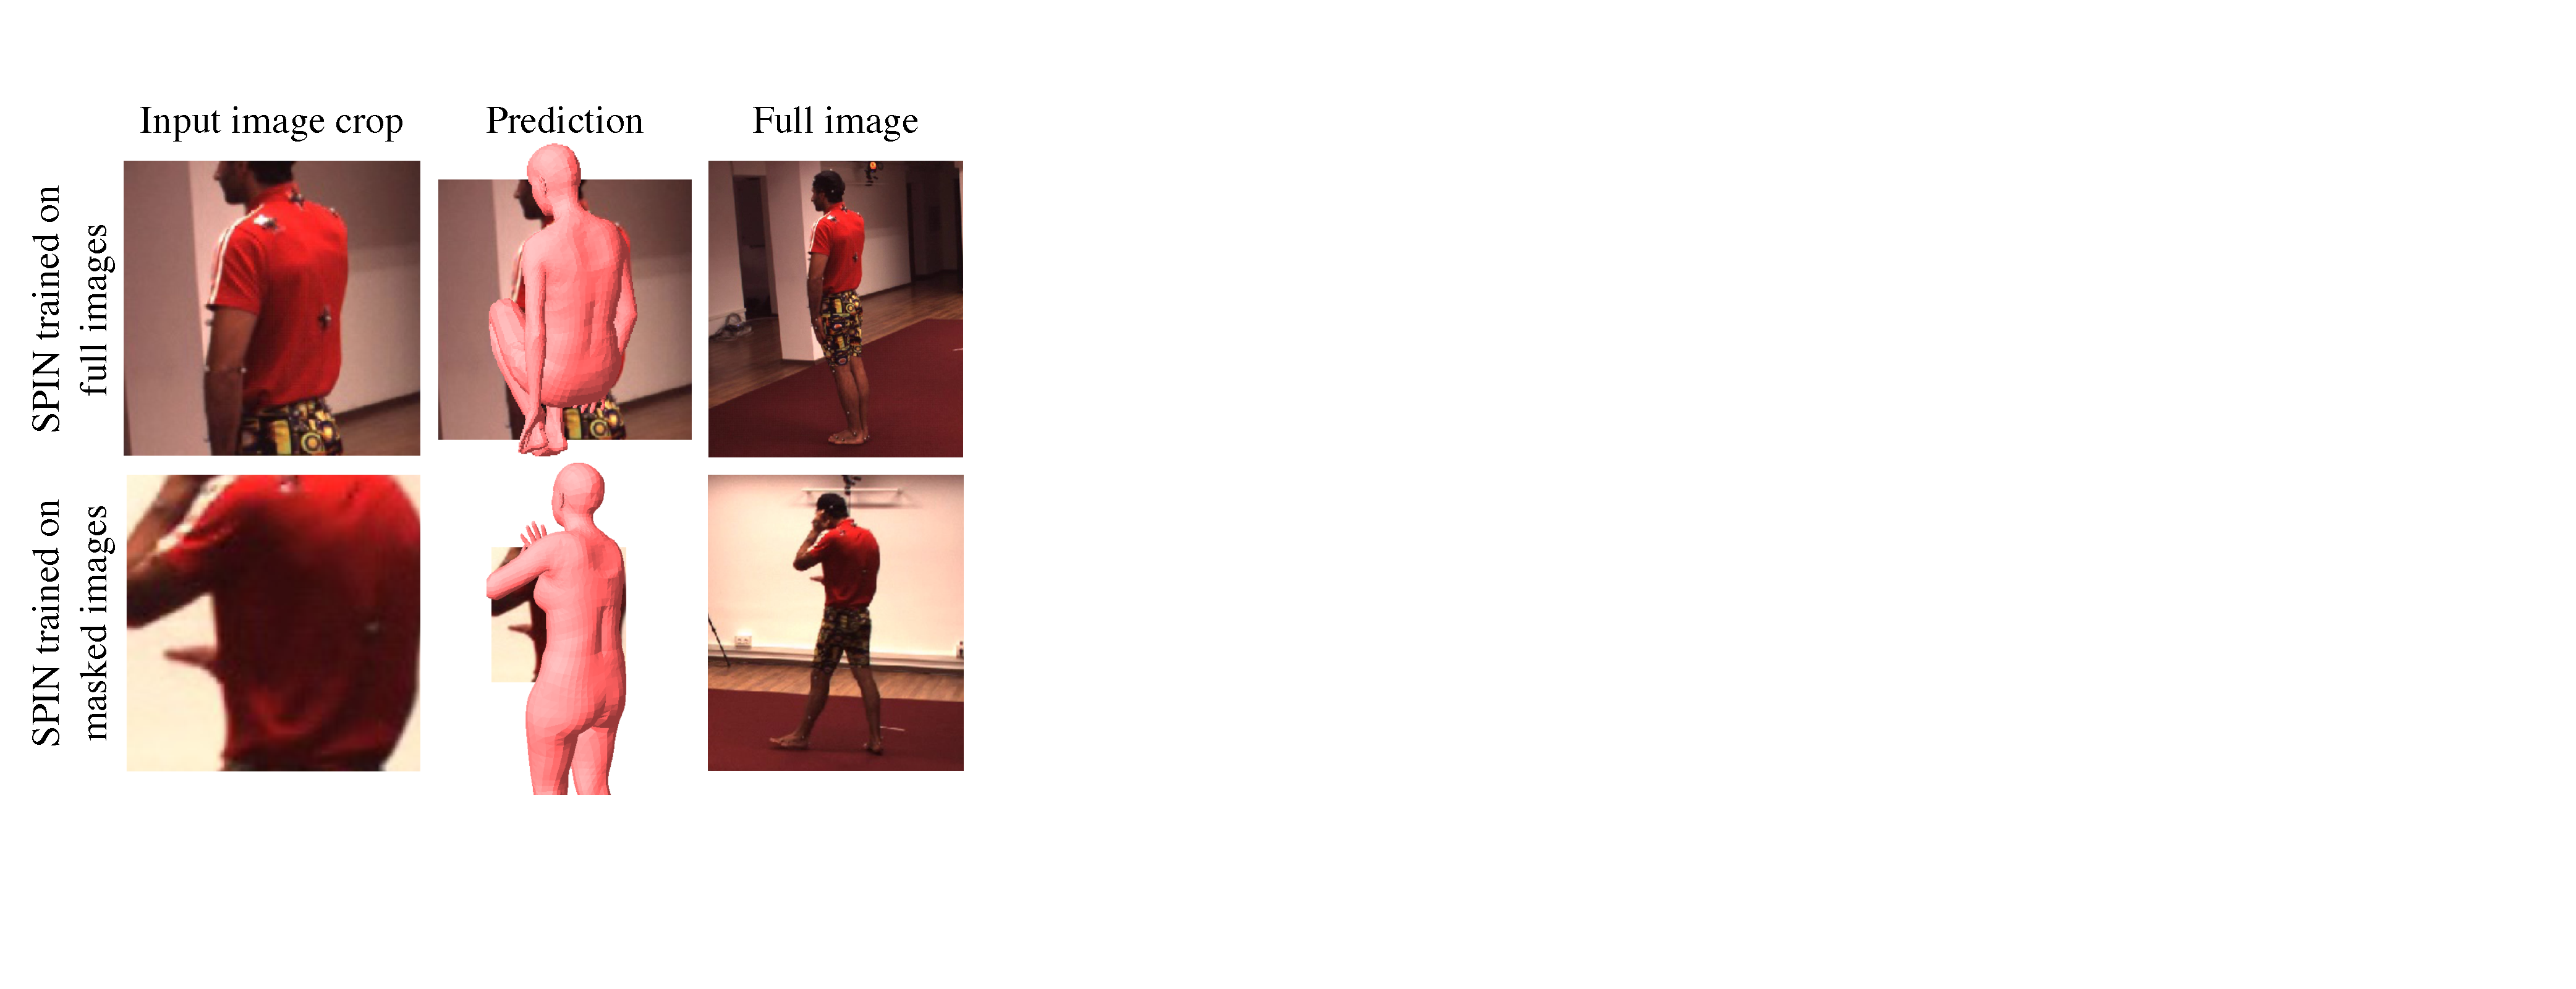
\includegraphics[width=\linewidth]{failures/failure_summary_v2} %
    \caption{
        \textbf{Top}: Pretrained SPIN model tested on an ambiguous example, \textbf{Bottom}: SPIN model after fine-tuning to ambiguous examples. Note the network tends to regress to the mean over plausible poses, shown by predicting the missing legs vertically downward --- arguably the average position over the training dataset.}\label{fig:issues}
\end{figure}


\subsection{Modelling ambiguities in 3D reconstruction}

Several previous papers have looked at the problem of modelling ambiguous 3D human pose reconstructions. Early work includes~\citet{kinematic-jump-processes}, ~\citet{tracking-3d-human-figures} and \citet{density-prop}. % TODO: much more here.

% To be fair, we don't learn a prior directly on the SMPL parameters.

% They model distributions conditioned on the parent of each joint in the kinematic tree and show that this prior can be used to obtain improved parametric fits.
More recently,~\citet{akhter15pose-conditioned} learn a prior over human skeleton joint angles (but not directly a prior on the SMPL parameters) from a MoCap dataset.~\citet{li19generating} use the Mixture Density Networks model of~\cite{bishop94mixture} to capture ambiguous 3D reconstructions of sparse human body keypoints directly in physical space.
\citet{sharma19monocular} learn a conditional variational auto-encoder to model ambiguous reconstructions as a posterior distribution; they also propose two scoring methods to extract a single 3D reconstruction from the distribution.
\citet{cheng19occlusion-aware} tackle the problem of video 3D reconstruction in the presence of occlusions, and show that temporal cues can be used to disambiguate the solution.
While our method is similar in the goal of correctly handling the prediction uncertainty, we differ by applying our method to predicting \emph{full mesh} of the human body.
This is arguably a more challenging scenario due to the increased complexity of the desired 3D shape.
% TODO: add Ignas' work

% TODO: integrate this
Compared to these works, we also make a simple but important contribution of modelling ambiguity in the space of 3D model parameters.
Existing approaches, such as Mixture Density Networks~\cite{bishop94mixture,li19generating}, output instead a distribution on the reconstructed 3D location of a finite set of human body joints.
This is straightforward, but difficult to extend to full 3D meshes.
Instead, we argue that the parameters of the 3D model offer a better space for coding not just 3D shapes and poses, but also their ambiguities.
As far as we could determine, we are the first to model ambiguous reconstructions directly in the space of human body model parameters.



% Finally,~\citet{cheng19occlusion-aware} tackle the problem of video 3D reconstruction in the presence of occlusions, and show that temporal cues can be used to disambiguate the solution.
% While our method is similar in the goal of correctly handling the prediction uncertainty, we differ by applying our method to predicting \emph{full mesh} of the human body.
% This is arguably a more challenging scenario due to the increased complexity of the desired 3D shape.

% Several previous papers have looked at the problem of modelling ambiguity in 3D human pose reconstruction. Early work includes~\citet{kinematic-jump-processes}, ~\citet{tracking-3d-human-figures} and \citet{density-prop}. More recently, ~\citet{akhter15pose-conditioned} learn a prior over human skeleton joint angles from a MoCap dataset.
% %(but not directly a prior on the SMPL parameters)
% % They model distributions conditioned on the parent of each joint in the kinematic tree and show that this prior can be used to obtain improved parametric fits.
% More recently,~\citet{li19generating} use the Mixture Density Networks model of~\cite{bishop94mixture} to capture ambiguous 3D reconstructions of sparse human body keypoints directly in physical space.
% \citet{sharma19monocular} learn a conditional variational auto-encoder to model ambiguous reconstructions as a posterior distribution; they also propose two scoring methods to extract a single 3D reconstruction from the distribution.




\subsubsection{VAE}
% BicycleGan etc.
\subsubsection{MDN}
\subsubsection{Min-of-N}

Our primary contribution is to introduce a principled multi-hypothesis framework to model the ambiguities in monocular pose recovery.
In the literature, such multiple-hypotheses networks are often trained with a so-called \emph{best-of-$M$} loss --- namely, during training, the loss is incurred only by the best of the $M$ hypothesis, back-propagating gradients from that alone~\cite{guzman2012multiple}.
In this work we opt for the \emph{best-of-$M$} approach since it has been show to outperform  alternatives (such as variational auto-encoders or mixture density networks) in tasks that are similar to our 3D human pose recovery, and which have constrained output spaces \cite{rupprecht17learning}.


% We also make an important contribution to better optimize our multi-hypothesis predictions.

\subsection{Overcoming limitations with best-of-$M$ frameworks}

A major drawback of the \emph{best-of-$M$} approach is that it only guarantees that \emph{one} of the hypotheses lies close to the correct solution; however, it says nothing about the plausibility, or lack thereof, of the \emph{other} $M-1$ hypotheses, which can be of arbitrarily poor quality.
% TODO: Integrate this
\footnote{
Theoretically, best-of-$M$ can minimize its loss by quantizing optimally (in the sense of minimum expected distortion) the posterior distribution, which would be desirable for coverage.
However, this is \emph{not} the only solution that optimizes the best-of-$M$ training loss, as in the end it is sufficient that \emph{one} hypothesis per training sample is close to the ground truth.
In fact, this is exactly what happens; for instance, during training hypotheses in best-of-$M$ are known to easily become degenerate and `die off', a clear symptom of this problem.
}
%
Not only does this mean that most of the hypotheses may be uninformative, but in an application it is impossible to determine \emph{which} hypothesis should be used, leaving open the possibility of selecting a `bad' one.
This has also a detrimental effect during learning because it makes gradients sparse as prediction errors are back-propagated only through one of the $M$ hypotheses for each training image.

In order to address these issues, a first contribution in this chapter is a \emph{hypothesis reprojection loss} that forces each member of the multi-hypothesis set to correctly reproject to 2D image keypoint annotations.
The main benefit is to constrain the \emph{whole} predicted set of meshes to be consistent with the observed image, not just the best hypothesis, also addressing gradient sparsity.

Next, another drawback of the best-of-{$M$} pipeline is to be tied to a particular value of $M$, whereas in applications it is useful to be able to tune the number of hypotheses. In the standard best-of-{$M$} implementation, this would necessitate completely retraining the network with the updated value of $M$. 
Furthermore, minimizing the reprojection loss makes hypotheses geometrically consistent with the observation, but not necessarily likely.
The second contribution is therefore to improve the flexibility of best-of-$M$ models by allowing them to output any smaller number $n<M$ of hypotheses while at the same time making these hypotheses \emph{more representative of likely} poses.
The new method, referred to henceforth as $n$-quantized-best-of-$M$, does so by quantizing the best-of-$M$ model to output weighed by a \emph{explicit pose prior}, learned by means of normalizing flows.

\subsection{Methods to learn a 3D articulated pose prior}

% Harp back to the previous chapter talking about gaussian pose priors etc.

There are a number of techniques in the literature for building precise priors over human pose deformation. A common formulation, relied upon in previous chapters, is to impose a unimodal Gaussian on the 3D kinematic tree rotations. The mean and covariance parameters can either be obtained from the 3D scans used to construct the morphable model, or alternatively from a separate 3D dataset (e.g. CMU) which exhibits a wider range of motion. Alternative priors have been designed to specifically penalize ``interpenetration'', a phenomenon that a body part self-intersects the mesh or a prior that specifically penalizes ``out-of-range'' rotations. 

Recently, more expressive 3D pose priors have been designed based on modern deep laerning advancements. Kanazawa et al.~\cite{xxx} propose a method that uses a per-part discriminator to ensure network-predicted 3D models lie on a manifold of plausible bodies. In addition, VAE methods have been proposed which constrain poses to a Gaussian parameterized by higher-level features. % CITE 
Concurrently to the work in this chapter, priors have been built over 3D human pose using normalizing flows. In particular, ~\citet{xu-2020-cvpr} release a prior for their new GHUM/GHUML model, and~\citet{weakly-supervised-normflow} build a prior on SMPL joint angles to constrain their weakly-supervised network. The prior introduced in this chapter differs slightly as it is learnt on 3D morphable model joint locations, rather than the Rodrigues rotations.

% In order to do so, since best-of-$M$ lacks an explicit n\emph{prior} over plausible human body poses, thus resulting in an optimal coverage of the \emph{likely} solutions.

%an arbitrary number of $n<M$ hypotheses that optimally cover the set of plausible poses.



\subsection{Sourcing datasets for training and evaluation}

The method described in this chapter focuses on modelling ambiguities in 3D reconstructions using a min-of-$M$ loss. To train such a model, gradients are propagated through the best hypothesis -- in this case, the closest to a 3D ground truth mesh. Consequently, a dataset of images with corresponding 3D annotations is required. As previously described, such datasets are limited in number and size for animals, although the RGBD Dog dataset is suitable for this purpose. It is thought likely that the growing interest in 3D animal reconstruction will result in new datasets being made available shortly, and the method described here can be evaluated shortly. In the mean time, in order to test the quality of reconstruction methods, the method is extensively evaluated against competitive 3D human reconstruction benchmarks.

\subsection{System overview}
To summarise, our key contributions are as follows.
First, we deal with the challenge of 3D mesh reconstruction for articulated objects such as humans in \emph{ambiguous} scenarios.
Second, we introduce a \emph{$n$-quantized-best-of-$M$} mechanism to allow best-of-$M$ models to generate an arbitrary number of $n<M$ predictions.
Third, we introduce a mode-wise re-projection loss for multi-hypothesis prediction, to ensure that predicted hypotheses are \emph{all} consistent with the input.

Empirically, we achieve state-of-the-art monocular mesh recovery accuracy on Human36M, its more challenging version augmented with heavy occlusions, and the 3DPW datasets.
Our ablation study validates each of our modelling choices, demonstrating their positive effect.

\begin{figure*}[t]
\def\bb{\rule{2in}{0pt}\rule{0pt}{1in}}
\begin{center}
% \includegraphics[width=\linewidth,trim=0 170 70 0,clip ]{method/overview_v3.pdf}
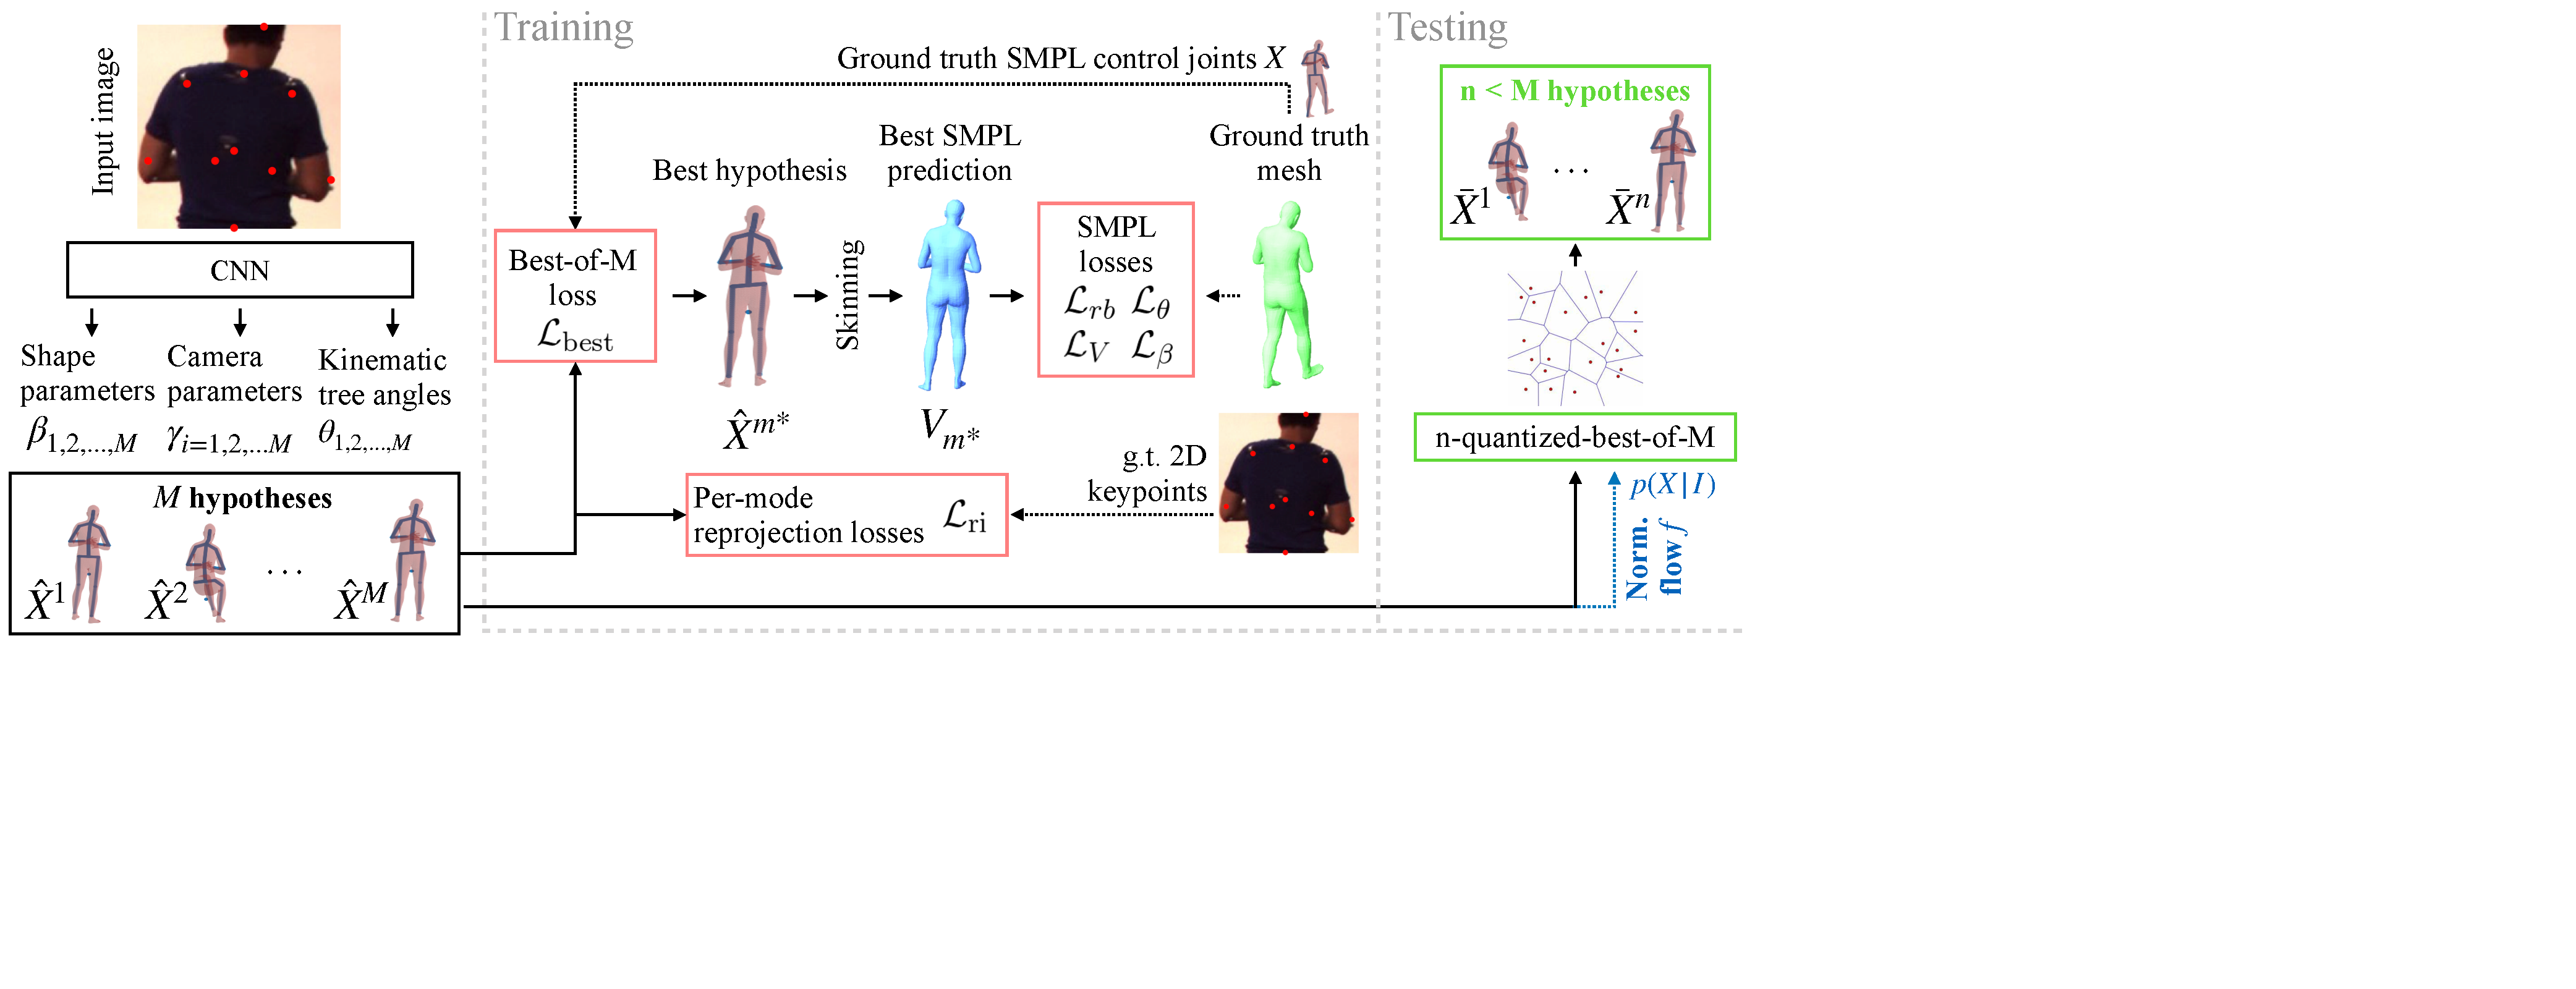
\includegraphics[width=\linewidth]{method/overview_v6.pdf}
\end{center}
\caption{\textbf{Overview of our method.}
Given a single image of a human, during training, our method produces multiple skeleton hypotheses $\{\hat Y^i\}_{i=1}^M$ that enter a Best-of-$M$ loss which selects the representative $\hat Y^{m^*}$ which most accurately matches the ground truth 3D control joints $Y$. 
% The camera parameters together with a skinned SMPL mesh enter the final set of SMPL losses.
At test time, we sample an arbitrary number of $n<M$ hypotheses by quantizing the set $\{\hat Y^i\}$ that is assumed to be sampled from the probability distribution $p(Y|I)$ modeled with normalizing flow $f$.
}\label{fig:arch_diagram}
\end{figure*}